\chapter{Introducción}
\label{cap:introduccion}
\begin{resumen}
	En este capítulo abordaremos la relevancia de la IA en el ámbito médico, describiremos los objetivos y el alcance del trabajo, y presentaremos la estructura general del documento.
\end{resumen}

\section{Fundamentos del electrocardiograma}
Un electrocardiograma (ECG) es una prueba diagnóstica no invasiva que registra la actividad eléctrica del corazón a lo largo del tiempo. Mediante la colocación de electrodos en puntos específicos del cuerpo (usualmente diez), se captan variaciones en los potenciales eléctricos producidos por el músculo cardíaco \citep{ribeiro}. Estas variaciones se reflejan en la forma de ondas y complejos (P, QRS, T), cuya interpretación permite identificar diversas patologías. Aunque estas mediciones pueden hacerse de diversas formas, lo habitual es medir la diferencia de potencial entre doce pares de electrodos. Cada una de estas mediciones genera una señal, que recibe el nombre de derivación.

Dado que no es posible recoger una cantidad continua de mediciones en el tiempo, se toma una cantidad de mediciones finita a una frecuencia específica (usualmente de 100Hz a 500Hz, dependiendo de la precisión del aparato medidor). Por tanto un ECG puede almacenarse en doce vectores de igual tamaño (variable dependiendo de la duración y frecuencia de la prueba). En la Figura \ref{fig:ecg} podemos ver un ejemplo de electrocardiograma (extraido de \cite{ptbxldb} y dibujado mediante la librería de python \emph{\text{ecg\_plot}}).

\begin{figure}[t]
	\setlength{\fboxsep}{0pt}%
	\fbox{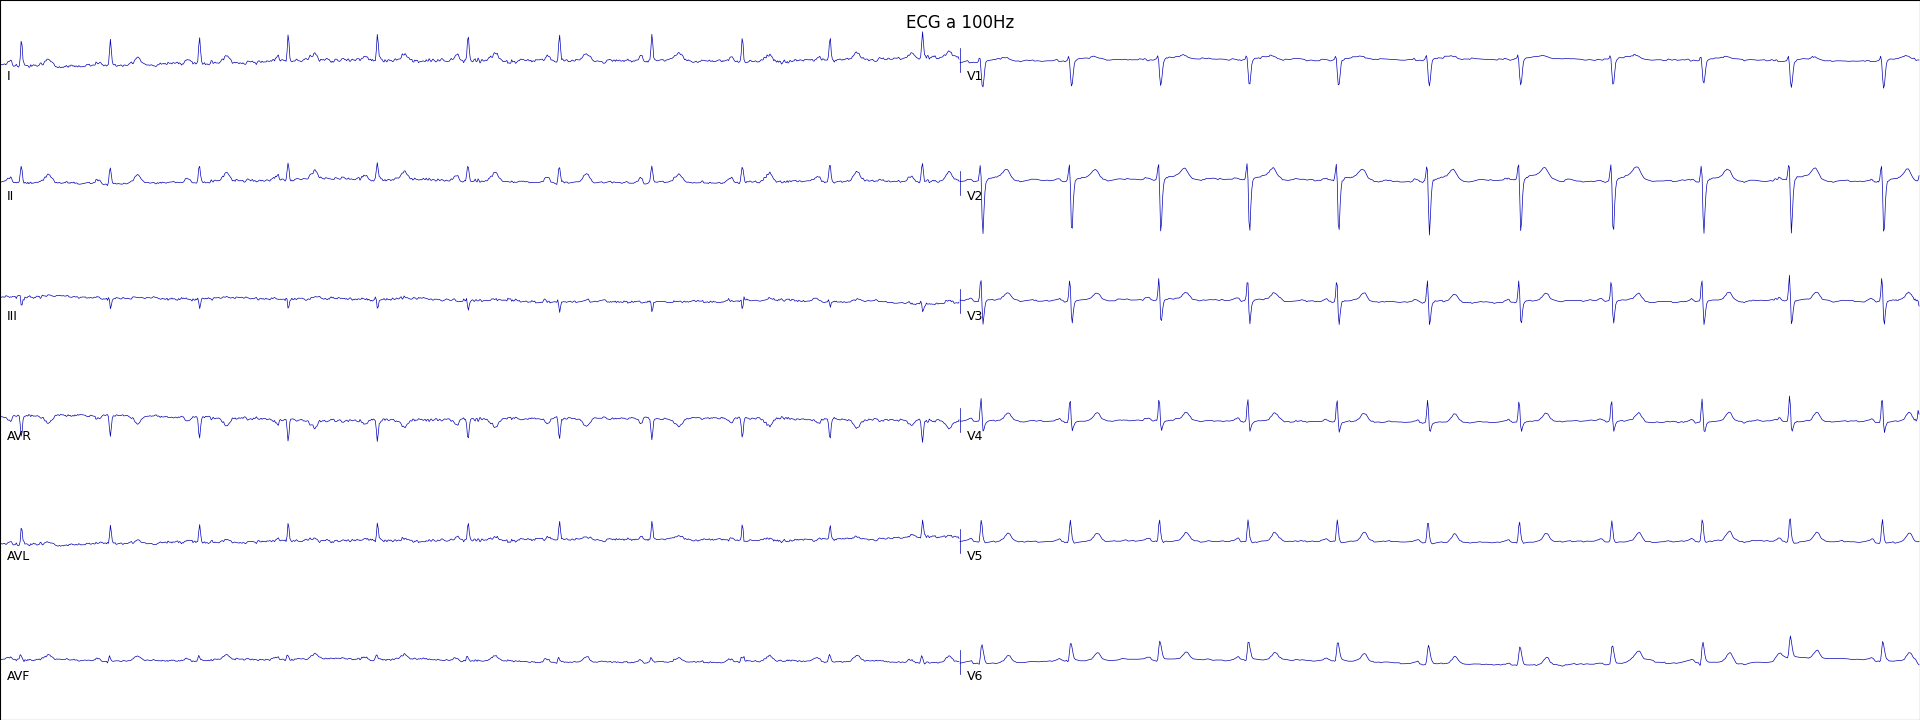
\includegraphics[width=\linewidth]{../Codigo/out/ecg100.png}}
	\fbox{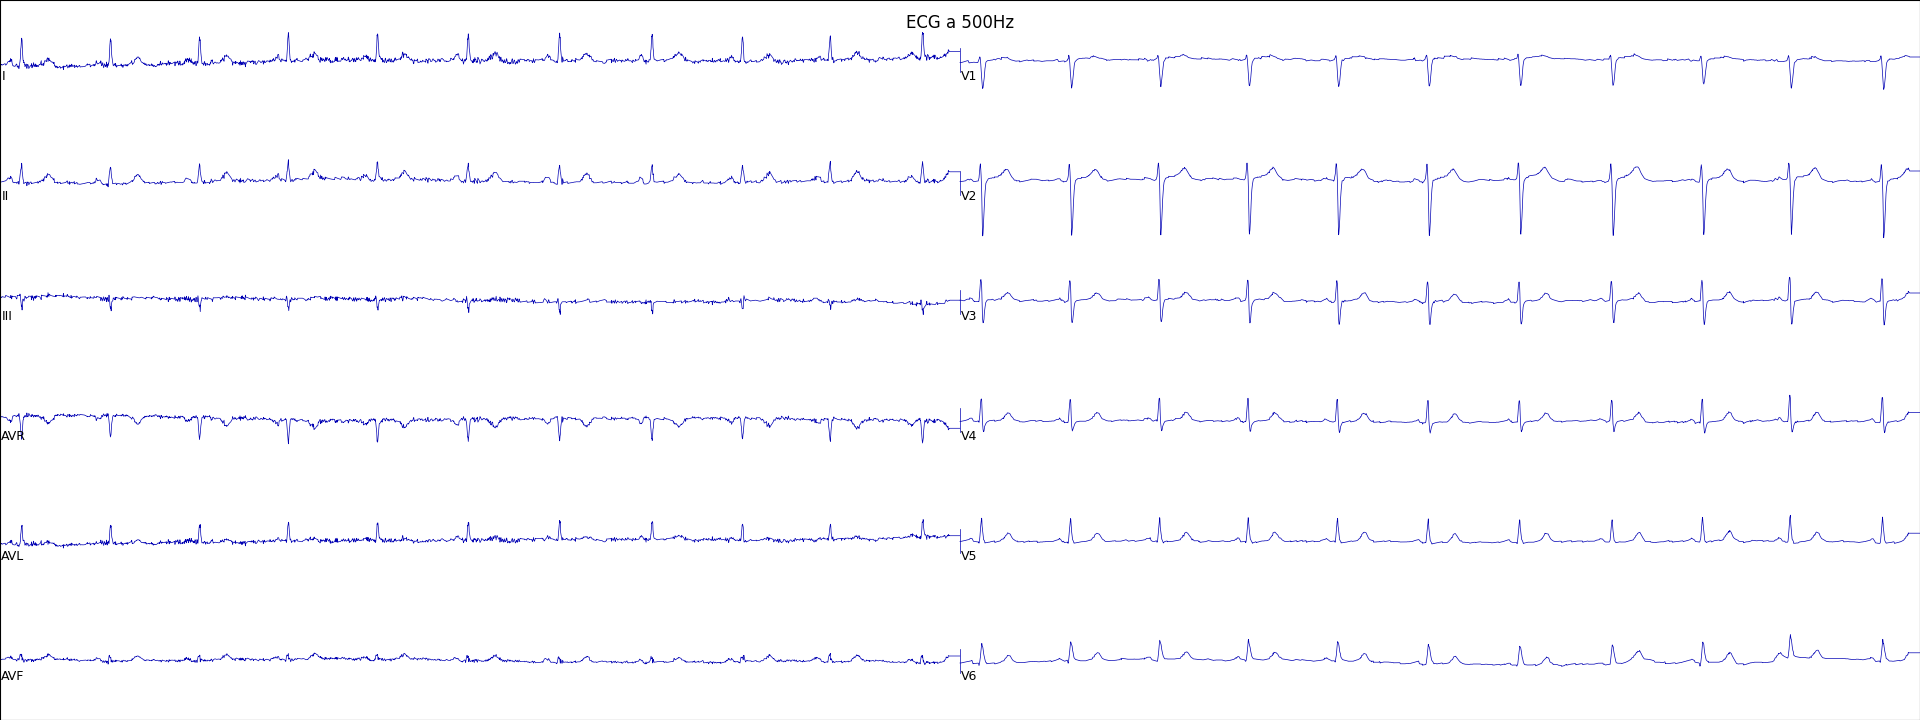
\includegraphics[width=\linewidth]{../Codigo/out/ecg500.png}}
	\caption{ECG de 12 derivaciones tomado a 100Hz (arriba) y 500Hz (abajo).}
	\label{fig:ecg}
\end{figure}

La frecuencia a la que se mide un ECG es muy importante. Si tiene una mayor frecuencia, la onda se puede ver con una mayor resolución, lo que permite detectar mejor las posibles anomalías. No obstante, además de que un aparato con capacidad de medir a más resolución es más complejo y caro, hay otras desventajas de tener una frecuencia muy alta. Una mayor frecuencia implica que para almacenar un ECG de la misma duración necesitamos más memoria, y será computacionalmente más costoso cualquier tipo de procesamiento o análisis que queramos realizar sobre este.

La relevancia clínica del ECG es enorme, además de ser una prueba de bajo coste y gran disponibilidad, el electrocardiograma constituye el primer paso para la detección de anomalías cardíacas en servicios de urgencias, consultas de atención primaria y especializadas. De acuerdo con la Organización Mundial de la Salud (OMS), las enfermedades cardiovasculares representan una de las principales causas de mortalidad a nivel global \citep{whocvd}; por ello, optimizar su diagnóstico temprano a través de métodos automatizados de análisis y clasificación puede tener un impacto significativo en la mejora de la salud pública.

En este contexto, se han desarrollado modelos de \emph{Deep Learning} muy precisos para el diagnóstico interpretable de anomalías cardíacas \citep{lu2024decoding}. A lo largo de este capítulo se profundizará en aspectos esenciales de la señal, se expondrán los fundamentos de las ondas principales y se describirán las bases de datos de ECGs más utilizadas para la investigación.

\subsection{Ondas y segmentos principales}

En la Figura \ref{fig:latido} se muestra un trazado típico de un ECG con etiquetas para cada onda y segmento. A grandes rasgos se pueden distinguir:
\begin{itemize}
	\item \textbf{Onda P}: la primera elevación relativamente pequeña.
	\item  \textbf{Complejo QRS}: El conjunto de picos y valles centrales, normalmente lo más destacado.
	\item \textbf{Onda T}: La elevación posterior que aparece después del complejo QRS.
	\item \textbf{Segmento ST}: La sección entre el final del complejo QRS y el inicio de la onda T.
	\item \textbf{Intervalo PR}: El espacio desde el inicio de la onda P hasta el comienzo del complejo QRS.
	\item \textbf{Intervalo QT}: El espacio desde el inicio de la onda Q hasta el final de la onda T.
	\item \textbf{Segmento PR}: La sección entre el final de la onda P y el comiendo del complejo QRS.
\end{itemize}

\begin{figure}
	\centering
	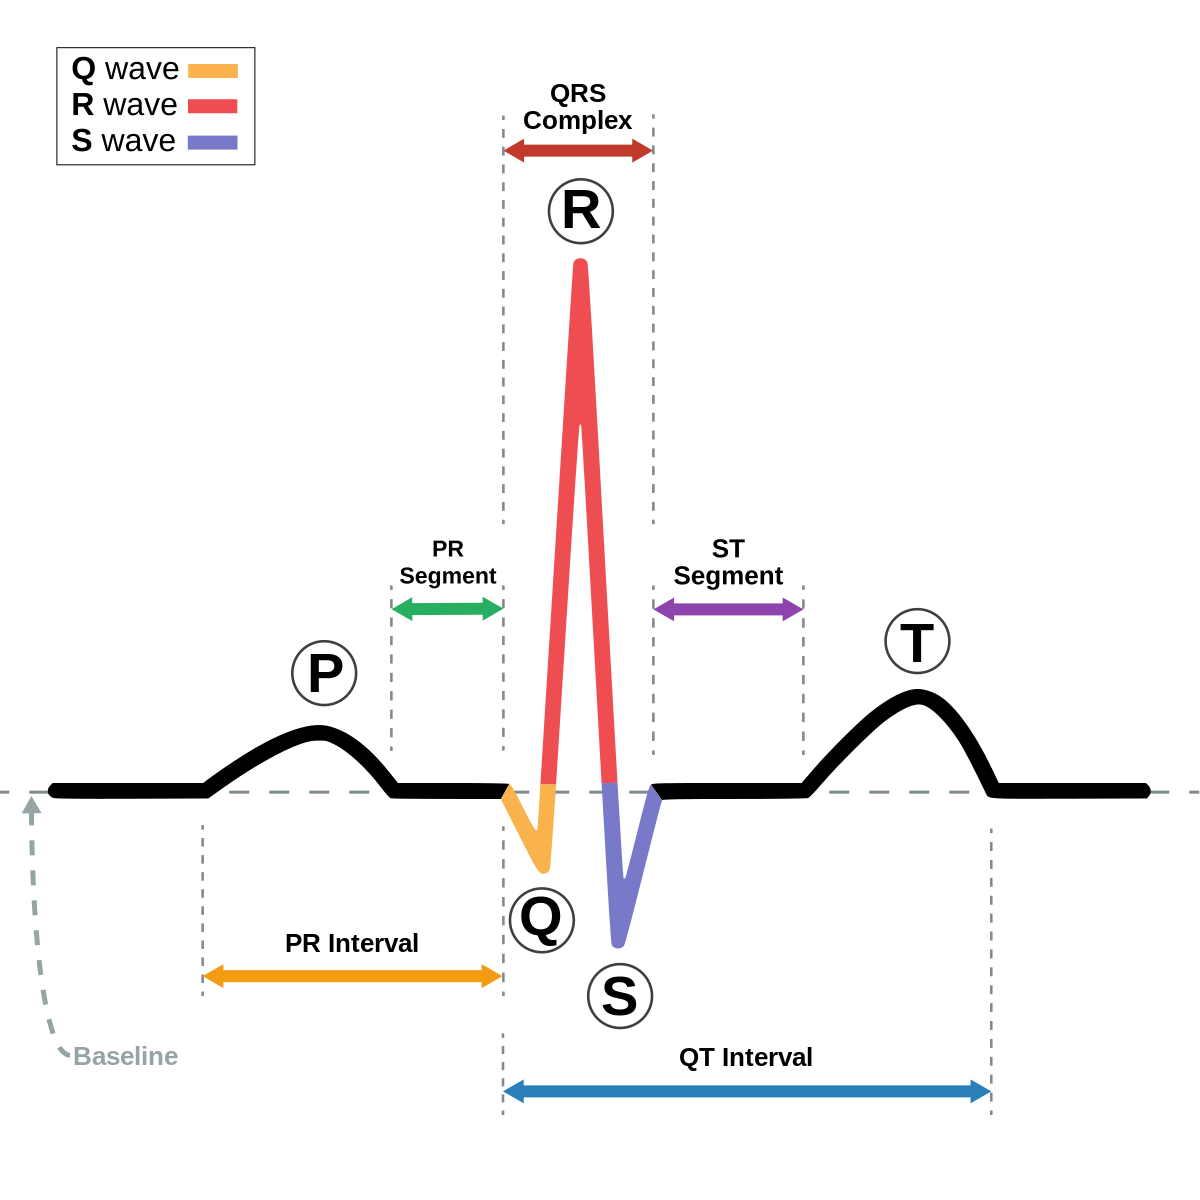
\includegraphics[width=0.5\textwidth]{Imagenes/Vectorial/latido.png}
	\caption{Ejemplo de ECG con etiquetas en P, QRS, T, ST y PR. Fuente: \cite{latido_img}}
	\label{fig:latido}
\end{figure}

Aunque cada uno de estos componentes tiene implicaciones fisiológicas y diagnósticas, en este trabajo no entraremos en ellos, ya que el conocimiento profundo de los procesos cardíacos que generan cada onda no es necesario para las técnicas de análisis y clasificación que utilizaremos. Para una descripción en detalle de las partes de un ECG, así como de la relación con los movimientos del músculo cardíaco, el lector puede referirse a \textbf{Manual de Electrocardiografía Básica} \cite{manualelectro}.

\subsection{Principales anomalías en un ECG}

Existen numerosas anomalías en un ECG que pueden reflejar alteraciones en la función cardíaca. En este trabajo, agruparemos las anomalías de la misma forma en la que están agrupadas en la base de datos elegida, que podemos ver en la Sección \ref{subsec:anomalias}.


\section{Motivación}
La Inteligencia Artificial (IA) ha transformado numerosos campos. En particular, la medicina ha experimentado avances significativos mediante la aplicación de la inteligencia artificial al diagnóstico y análisis de datos. Uno de los campos más prometedores es el de la interpretación automatizada de señales en un ECG, fundamentales para la detección temprana de enfermedades cardíacas. Las enfermedades cardiovasculares son una de las principales causas de muerte a nivel global \citep{whocvd}, lo que subraya la necesidad de métodos rápidos y precisos para su diagnóstico.

El análisis de ECGs ha sido históricamente una tarea realizada por profesionales de la salud, como cardiólogos, debido a la complejidad y variabilidad de las señales y de la interpretación de estas. Sin embargo, este proceso es lento, costoso y depende en gran medida de la experiencia del especialista. Con la adopción de modelos de \emph{Deep Learning}, como las redes neuronales convolucionales (CNN), surge la oportunidad de automatizar y mejorar este análisis, proporcionando resultados rápidos, y en muchos casos, comparables a los obtenidos por expertos humanos \citep{hannun_cardiologist_2019}. Este enfoque no solo promete aumentar la eficiencia del diagnóstico, sino también mejorar la precisión y reducir la carga de trabajo del personal médico.

Sin embargo, los médicos se han mostrado reacios a utilizar estas tecnologías debido a que en muchas ocasiones, por ser modelos predictivos que no proporcionan explicaciones (modelos de caja negra), no pueden comprender su funcionamiento. Para que este tipo de herramientas genere confianza en entornos clínicos y cumpla con los estándares de calidad y ética, es fundamental que sean explicables \citep{Molnar2019}. La explicabilidad de los modelos de IA hace posible comprender y justificar las decisiones tomadas durante el análisis de la señal cardíaca, un factor crítico en aplicaciones de alto impacto como la medicina, donde un error puede afectar directamente a la salud de los pacientes \citep{Goodman2017}.

Si bien se ha realizado una cantidad significativa de investigación en el campo de análisis y predicción de riesgos a partir de ECGs (por ejemplo \cite{Ribeiro}), no son tantos los trabajos que hay que ponen el foco en tener modelos explicables, lo que es muy importante (como señalábamos en el párrafo anterior) para que estos modelos sean realmente utilizados. Creemos que, si los modelos transformados obtienen resultados similares (o mejores) que el modelo original, estos podrían dar mejores resultados a la hora de aplicar técnicas de explicaión.

\com{Esto lo he añadido para resaltar el motivo de utilizar transformadas, ver si dan mejores explicaciones. pero claro, entre que el modelo no da buenos resultados con las transformadas y que hay limitaciones técnicas que descubrimos más adelante, no hemos llegado a probar explicar las transformadas. Esta es la última revisión del trabajo, así que creo que o dejo este último párrafo o lo quito, pero no quiero estar haciendo cambios de redacción mayores (salvo erratas o meteduras de pata similares) a estas alturas.}

A lo largo de este trabajo, exploraremos diversas arquitecturas de redes neuronales y técnicas de transformación de señales para clasificar y detectar anomalías en ECGs, con el objetivo de desarrollar y mejorar un modelo clasificador de ECGs en cuatro grupos de anomalías cardíacas. Además, incorporaremos métodos de explicabilidad para que los resultados del modelo puedan ser interpretados y validados por profesionales de la salud, lo que es esencial para la adopción clínica de estas tecnologías.

\section{Objetivos}
El principal objetivo de este trabajo es modificar, entrenar y evaluar el modelo propuesto originalmente por \cite{ribeiro} (en adelante, `\emph{gold standard}'), aplicándolo sobre una base de datos pública. Para lograrlo, introduciremos una modificacion en la capa de entrada del modelo que permita la inclusión de transformadas (por ejemplo STFT o CWT) a fin de explorar si la conversión de la señal en distintas representaciones puede mejorar el rendimiento. No obstante, no se realizan cambios en la arquitectura interna del modelo.

Con base en lo anterior, los objetivos específicos son:

\begin{enumerate}
	\item \textbf{Entrenar el \emph{gold standard}} con una base de datos pública.
	\item \textbf{Modificar el \emph{gold standard}} para que admita transformaciones de la señal, posibilitando el entrenamiento de versiones alternativas del modelo con datos transformados.
	\item \textbf{Comparar el rendimiento} de cada variante con el \emph{gold standard} mediante métricas como F1-Score, analizando si las transformaciones resultan o no beneficiosas.
	\item \textbf{Aplicar un método de explicabilidad} para que un especialista pueda comprender qué partes de la señal de un ECG influyen en la predicción.
\end{enumerate}

\section{Estructura del documento}
El presente documento se organiza en seis capítulos, cuyo contenido se describe a continuación:
\begin{itemize}
	\item \textbf{Capítulo 2: Estado del arte} \\
	Se exponen los conceptos básicos sobre electrocardiogramas, resaltando la importancia de sus ondas (P, QRS, T) y las anomalías más comunes que se suelen detectar. Asimismo, se revisa la literatura relacionada con el uso de redes neuronales en el análisis de ECGs y se describen bases de datos relevantes (como PTB-XL).
	
	\item  \textbf{Capítulo 3: Metodología y preparación de datos} \\
	Se detalla el proceso de tratamiento de los ECGs, incluyendo la división en conjuntos de entrenamiento, validación y prueba. Además, se describen las métricas utilizadas para evaluar los modelos y las transformaciones empleadas.
	
	\item \textbf{Capítulo 4: Entrenamiento y resultados}\\
	Se explican las condiciones de entrenamiento de cada modelo (incluyendo las modificaciones del \emph{gold standard}) y las librerías utilizadas y se presentan y comparan los resultados cuantitativos obtenidos por las métricas.
	
	\item \textbf{Capítulo 5: Explicabilidad}\\
	Se describe el método de explicabilidad basado en \emph{saliency maps} de gradientes aplicado al modelo de Ribeiro. Asimismo, se incluye la perspectiva de un médico especialista que analiza las explicaciones generadas y se reflexiona sobre el método y posibles mejoras.
	
	\item \textbf{Capítulo 6: Conclusiones y trabajo futuro}\\
	Se integran las conclusiones derivadas de los resultados, valorando en qué medida se han cumplido los objetivos planteados. Además, se señalan las principales contribuciones de este trabajo y se proponen líneas de investigación futuras (como la inclusión de capas Conv2D).
\end{itemize}

Por último, se incluye un apartado de bibliografía, donde se recogen todas las fuentes consultadas a lo largo del documento, así como un anexo con el código utilizado\footnote{Todo el contenido de este trabajo puede encontrarse en \href{https://github.com/NotNoe/TFG-Info}{este repositorio de github}.} y otro con la totalidad de librerías instaladas en el entorno de \emph{Python} sobre el que se ejecutó el código.
